% ===================================================================
\section{Data and Methodology}\label{sec:data}
% ===================================================================
This section sets out the foundations of the empirical design: the data we use, the
choices that govern the donor pool and the estimation windows, the estimators that
proxy the counterfactual, and the validation battery that defends the estimate. Two
themes recur and both follow from the factor model of Section~\ref{sec:theory}. Donor
selection is an identification choice rather than a fit-maximising one, and the length
of the estimation window is itself a SUTVA consideration, not merely a sample-size one.
We describe here \emph{what} the pool and the methods are and \emph{why} they were
chosen; the donor-by-donor audit that adjudicates which candidates survive is deferred
to Section~\ref{sec:donoraudit}.

\subsection{Target and sources}
The target is the daily \emph{Europe Brent Spot Price FOB} (EIA series RBRTEd), in
USD per barrel, downloaded directly from the U.S.\ Energy Information Administration
\citep{eia_brent}. The donor candidates are 32 macro-financial series from Yahoo
Finance, and they are not an arbitrary collection: they are chosen to span the
asset classes through which the common factors of equation~\eqref{eq:factor} move Brent.
The 32 fall into seven broad categories---metals (6: copper, iron ore, silver, platinum,
palladium, gold), agriculturals (7: soybeans, wheat, corn, coffee, sugar, cotton, live
cattle), equities (3: S\&P~500, Nikkei~225, EM equities), foreign exchange (11: AUD, JPY,
CHF, CNY, INR, KRW, ZAR, MXN, EUR, GBP, and the dollar basket DXY), rates and credit
(3: the US 10-year yield, long Treasuries TLT, high-yield credit HYG), volatility (1: the
VIX), and crypto (1: Bitcoin). Metals and equities proxy the global industrial cycle, FX
the dollar and terms-of-trade channels, rates and credit the real-rate and risk-premium
factors, and volatility the risk-appetite factor, so the candidate set covers all five
drivers before any audit narrows it. The panel is updated incrementally so it keeps pace
with new data. Table~\ref{tab:sources} summarises the sources. All are public and
redistributable, and the panel is rebuilt from source on each run so the analysis is
reproducible against the latest available data (here, through 15~June~2026 for Brent,
the binding constraint given the EIA's roughly one-week publication lag, and
23~June~2026 for the donors).

\begin{table}[h]
\centering
\caption{Data sources.}
\label{tab:sources}
\begin{threeparttable}
\small
\begin{tabular}{@{}p{3.0cm}p{3.6cm}p{7.0cm}@{}}
\toprule
Object & Source & Contents \\
\midrule
Brent spot (target) & EIA, series RBRTEd & Europe Brent Spot FOB, USD/bbl, 1987--present\\
Donor candidates (32) & Yahoo Finance & Metals, agriculturals, equities, FX, rates, credit, volatility, crypto\\
\bottomrule
\end{tabular}
\begin{tablenotes}[flushleft]
\footnotesize
\item \textit{Notes.} All series are daily and publicly redistributable.
\end{tablenotes}
\end{threeparttable}
\end{table}

\subsection{Donor pool: selection criteria and the shared-pool choice}
Donor selection is central to identification (Section~\ref{sec:theory}), and it is
governed by an explicit set of criteria rather than by raw correlation with Brent. A
series qualifies only if it satisfies all four of the following:
\begin{enumerate}
\item \textbf{Common-factor co-movement.} It co-moves with Brent through the common
global factors of equation~\eqref{eq:factor}, not through the oil-specific term. This is
the positive case for inclusion: the pool is built to span the five drivers (global
industrial cycle, the dollar, real rates, risk appetite, China demand) so the synthetic
can reproduce Brent under any mix of them.
\item \textbf{No interference (SUTVA).} It is \emph{not} physically routed through the
disruption being attributed. This is the criterion that does the identifying work; it is
enforced by a per-event audit that classifies each candidate as Clean, Mild, or Heavy
according to its exposure to the focal event (Section~\ref{sec:donoraudit}).
\item \textbf{Liquidity.} It is liquid and daily-traded, with a public, redistributable
source.
\item \textbf{History.} It has sufficient pre-event history for the events under study.
\end{enumerate}

The central design choice concerns \emph{which} pool to carry across the two events. We
fit both Russia and Hormuz on a single shared pool, formed by retaining only the
candidates that are Clean for \textbf{Russia 2022}, the more demanding of the two audits.
Because the Russia strict-clean set is a subset of the Hormuz clean set, every member of
the shared pool stays clean for both events, so the same basket is a valid counterfactual
in each. The alternative, using each event's own maximal clean set, would maximise
within-event fit but would prevent the cross-event weight-transfer check that is the
strongest robustness test available with only two events (Section~\ref{sec:results}); we
prefer the shared pool and treat the sacrificed Hormuz-clean donors as the price of
comparability. The energy complex (WTI, refined products, petrocurrencies) is excluded
by construction under criterion (ii): it has the highest raw correlation with Brent but
loads on the very oil-specific shock $o_t$ we are trying to measure, so including it
would choose fit over identification. The donor-by-donor execution of this audit, the
resulting membership, and the empirical tests that confirm it are the subject of
Section~\ref{sec:donoraudit}; the full per-event catalog of all 32 candidates is
Table~\ref{tab:donoraudit} in Appendix~\ref{app:donoraudit}.

\subsection{Window selection}
The estimation window must be chosen, not maximised. For daily-traded benchmarks like
Brent and its donors, a longer pre-history is not automatically better. These series
pass through distinct market regimes, and a window that spans several of them risks
teaching the synthetic a donor--Brent relationship that no longer holds in the
projection period, a regime shift that re-enters as post-event interference and thus as
a SUTVA violation. Our first task was therefore to locate the longest pre-window that
contains \emph{no} prior shock or regime break, rather than the longest pre-window
available. Each event then has such a pre-window (for fitting) and a post-window (for
projecting the counterfactual), each $\sim$20 months. Following \citet{abadie2021}, the
Russia pre-window starts 2020-07-01, deliberately \emph{after} the March--May 2020
cluster (OPEC+ collapse, WTI-negative, acute COVID) that would otherwise impose an
abnormal factor loading. The Russia post-window is truncated at 2022-09-30, the last
business day before OPEC+'s October 2022 supply cut, a Brent-specific policy shock that
would confound the invasion premium. The Hormuz post-window extends to the latest
available data (2026-06-15). Table~\ref{tab:summary} reports summary statistics, and
Figure~\ref{fig:timeline} plots the full Brent series with both events and the shaded
pre- and post-windows. Brent roughly doubled after both focal shocks from a similar
$\sim$\$75 base, but from very different pre-event trajectories: a steep 2020--22 recovery
rally before Russia and a mild net decline through 2024--25 before Hormuz. This
trajectory asymmetry is what makes a na\"ive trend-extrapolation counterfactual
unreliable (Section~\ref{sec:results}).

\begin{table}[h]
\centering
\caption{Summary statistics of Brent spot, by event sample.}
\label{tab:summary}
\begin{threeparttable}
\small
\begin{tabular}{@{}llrrrrr@{}}
\toprule
Event & Segment & $n$ (days) & Mean & SD & Min & Max \\
\midrule
\multirow{3}{*}{Russia 2022}
 & Full sample & 572 & 75.95 & 24.76 & 36.33 & 133.18 \\
 & Pre-window  & 421 & 64.26 & 16.39 & 36.33 & 101.66 \\
 & Post-window & 151 & 108.54 & 11.37 & 82.55 & 133.18 \\
\addlinespace
\multirow{3}{*}{Hormuz 2026}
 & Full sample & 515 & 76.95 & 14.30 & 59.93 & 138.21 \\
 & Pre-window  & 443 & 72.08 & 6.58 & 59.93 & 88.66 \\
 & Post-window & 72  & 106.92 & 12.31 & 77.24 & 138.21 \\
\bottomrule
\end{tabular}
\begin{tablenotes}[flushleft]
\footnotesize
\item \textit{Notes.} Prices in USD/barrel. Pre/post split at $T_0$; Russia $T_0$=2022-02-24, Hormuz $T_0$=2026-02-28.
\end{tablenotes}
\end{threeparttable}
\end{table}

\begin{figure}[h]
\centering
\caption{Brent crude spot price and the curated event timeline, 2020--2026.}
\label{fig:timeline}
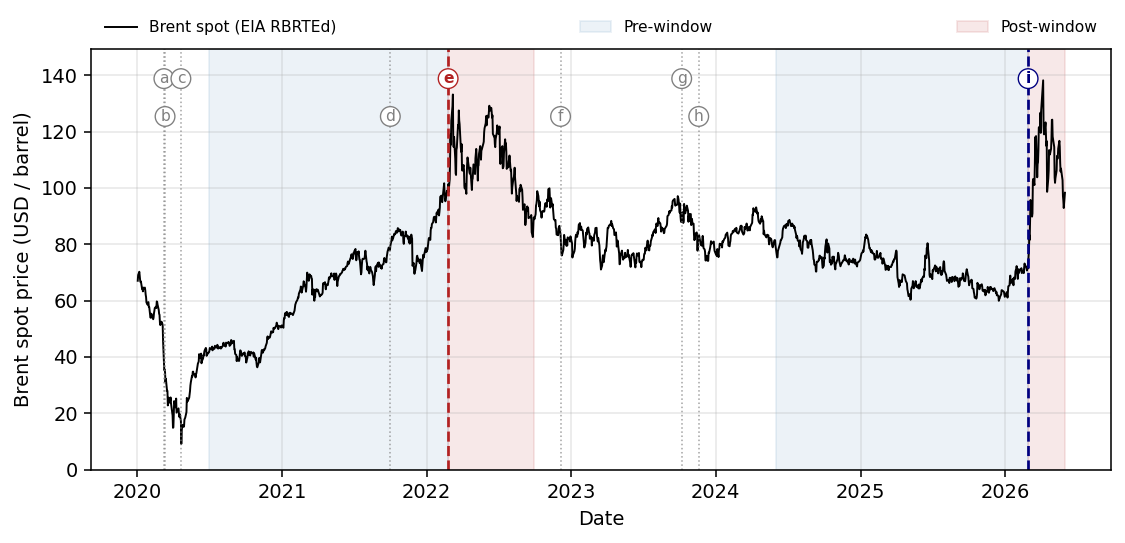
\includegraphics[width=0.92\textwidth]{figures/brent_timeline.png}

\smallskip
\begin{minipage}{0.92\textwidth}
\footnotesize \textit{Notes.} Lettered markers date the curated timeline events; the two
focal events (\textbf{e}, \textbf{i}) are bold dashed lines, the rest grey dotted.
(a)~Saudi--Russia price war, 8 Mar 2020; (b)~COVID-19 pandemic, 11 Mar 2020;
(c)~WTI-negative, 20 Apr 2020; (d)~energy-cycle reflation, 1 Oct 2021;
(e)~\textbf{Russia invades Ukraine, 24 Feb 2022}; (f)~Russia oil price cap, 5 Dec 2022;
(g)~Israel--Hamas war, 7 Oct 2023; (h)~Red Sea diversion, 19 Nov 2023;
(i)~\textbf{Strait of Hormuz crisis, 28 Feb 2026}. Shaded bands are each focal event's
preferred-specification estimation windows: blue the pre-window (fitting), red the
post-window (projection). \textit{Source:} Brent, EIA series RBRTEd; event timeline
curated by the authors (Appendix~\ref{app:donoraudit} for the donor-side audit).
\end{minipage}
\end{figure}

The two pre-windows differ in a way that matters later. The Russia pre-period is
volatile (SD~\$16.4, spanning the COVID recovery and the 2021 reflation rally), while the
Hormuz pre-period is much calmer (SD~\$6.6). This difference drives much of the contrast
in the two events' inference, because a volatile pre-period widens the placebo
distribution and weakens Russia's permutation test even though its magnitude is
well-documented.


\subsection{Estimators and the ensemble}\label{sec:methods}
A single specification cannot be trusted because the counterfactual's functional form is
unknown. Equation~\eqref{eq:factor} need not be linear in the donors, and the
convex-hull restriction of classical SCM may or may not bind. Rather than commit to one
form, we proxy the counterfactual with five estimators whose inductive biases bracket the
plausible cases (Table~\ref{tab:models}): a simplex-constrained average, a
ridge-extrapolating correction, a sparse signed regression, a nonlinear tree ensemble,
and a Bayesian linear model. An estimated premium that survives across biases this
different is far more likely to reflect a real effect than a single-model artefact. We
report the cross-model \emph{median} as the headline, which is robust to any one model
misbehaving, and the inter-quartile range as a model-uncertainty band that complements
each model's own within-model interval.
\begin{table}[t]
\centering
\caption{The five-estimator ensemble.}
\label{tab:models}
\begin{threeparttable}
\small
\begin{tabular}{@{}p{2.6cm}p{7.4cm}p{4.0cm}@{}}
\toprule
Estimator & Inductive bias & Reference \\
\midrule
Convex SCM & Non-negative donor weights summing to one, synthetic inside the donor convex hull & \citet{abadie2010}\\
Augmented SCM & Convex SCM plus ridge bias-correction, limited extrapolation outside the hull & \citet{benmichael2021}\\
Elastic net & Signed, sparse$+$ridge regression, lasso term drops donors entirely & \citet{doudchenko2016}\\
Gradient boosting (XGBoost) & Nonlinear, tree-based, captures interactions, cannot extrapolate beyond the training range & \citet{chenguestrin2016}\\
Bayesian ridge & Bayesian linear regression on donor levels (regression component of BSTS), conjugate Gaussian--Gamma prior & \citet{brodersen2015}\\
\bottomrule
\end{tabular}
\begin{tablenotes}[flushleft]
\footnotesize
\item \textit{Notes.} Each estimator contributes a distinct inductive bias; the headline is the cross-model median gap across the five.
\end{tablenotes}
\end{threeparttable}
\end{table}

All five estimators (Table~\ref{tab:models}) take the same input (log donor levels) and
target log Brent over the pre-window, then project the post-window counterfactual. The
two events are estimated entirely separately: they share the same 19-donor pool and the
same five-estimator pipeline, but each event trains its own models on its own pre-window,
so no parameter learned on one event is carried to the other. \emph{Convex SCM} solves
the classic nested optimisation: non-negative weights summing to one, chosen to minimise
pre-period RMSPE \citep{abadie2010}. \emph{Augmented SCM} adds a ridge penalty that
corrects for imperfect pre-fit and allows limited extrapolation \citep{benmichael2021}.
The \emph{elastic net} relaxes the simplex to signed, sparse coefficients
\citep{zouhastie2005,doudchenko2016}. \emph{XGBoost} fits shallow gradient-boosted trees
\citep{chenguestrin2016}, deliberately constrained (depth-2 stumps, strong
regularisation, row/column subsampling) for the small-sample regime. \emph{Bayesian
ridge} is a conjugate Bayesian linear regression on donor levels, the regression
component of BSTS \citep{brodersen2015}. Hyperparameters are tuned over small grids
(3--9 configurations) to bound the selection bias of \citet{cawley2010}; the convex SCM
has no tuned hyperparameter. Because the five estimators produce incommensurable weight vectors, a simplex for convex
SCM, signed unconstrained coefficients for the regressions, and no linear weights at all
for XGBoost, the ensemble operates on the \emph{gap series} each model implies rather
than on the weights. The headline at every $t$ is the cross-model median gap, with the
inter-quartile range as the model-uncertainty band.

A note on labelling: the fifth estimator is a Bayesian \emph{ridge} regression, not full
Bayesian structural time series. It implements only the regression-on-donors component
$\beta'x_t$ of \citet{brodersen2015} and omits the trend, seasonal, and spike-and-slab
selection components. At our sample size, and with no strong weekly seasonality, the
regression term carries most of the signal, but the model is best read as a
Bayesian-flavoured diversifier rather than a state-space causal-impact estimator
(Appendix~\ref{app:bsts}).

\subsection{Validation battery and its logic}
A credible SCM estimate must clear three levels \citep{abadie2021}: pre-event fit, donor
identification, and inference. We organise the validation around these three levels and
run every test per model and per event.

The first level concerns \emph{fit}. Out-of-sample tracking is assessed by
expanding-window walk-forward cross-validation \citep{hyndman2018,bergmeir2012}. Its role
here is not model selection but evidence against over-fitting: a synthetic whose
out-of-sample pre-period tracking matches its in-sample tracking is reproducing a stable
donor--Brent relationship rather than memorising the pre-window, which is the empirical
content of the common-factor spanning assumption.

The second level concerns \emph{identification}, and is the donor-cleanliness battery
that defends the no-interference (SUTVA) assumption. Before any model is fit, each
donor's own return series is tested for a mean shift at $T_0$ using a permutation form of
the known-break test of \citet{chow1960} (rather than the unknown-break test of
\citet{andrews1993}, since the date is known), together with a Wilcoxon event-window test
\citep{brownwarner1985}; a donor is flagged if either rejects after Benjamini--Hochberg
FDR control \citep{benjaminihochberg1995}. Regime stability is checked with distance
correlation across pre-period thirds \citep{szekely2007} and with Bai--Perron break
dating \citep{baiperron1998,baiperron2003}, and an I(0)/I(1)-robust trend-break test
\citep{harvey2009,kpss1992} confirms that no donor's own trend breaks at either $T_0$.
This battery operates at the level of the individual donor, so its outcomes are reported
with the donor audit (Section~\ref{sec:donoraudit}) rather than here.


The third level concerns \emph{inference}. We run the in-space placebo, refitting each
donor as a placebo treated unit and ranking Brent's post/pre RMSPE ratio against the
resulting distribution \citep{abadie2010}, reading the permutation $p$-value with the
symmetry caveat of \citet{hahnshi2017}. We add the in-time placebo at a fake $T_0$ six
months early, formalised as the mixed placebo test of \citet{chenyan2023}, and a
leave-one-donor-out check. Two further benchmarks sit alongside the formal tests: a
deliberately contaminated set of na\"ive univariate counterfactuals (random walk, drift,
linear trend, and an AIC-selected ARIMA that reduces to a driftless random walk in both
events) as a floor, and the signed contamination-bias diagnostic of
equation~\eqref{eq:bias}. Following \citet{roth2022,rambachanroth2023}, we report and
interpret pre-period diagnostics rather than turning them into pass/fail thresholds, and
we do not auto-exclude flagged models, because the cross-model IQR is itself the
model-uncertainty band. Finally, where a model's pre-period gap series is not flat, we
report a drift-adjusted gap alongside the raw one. We fit an ordinary least-squares trend
to the pre-period gap, read off its slope $\hat\beta$ in percent per year, and subtract
the portion that this pre-existing drift would contribute over the post-window on its
own, namely $\hat\beta L$ percentage points for a post-window of length $L$ years. The
adjustment isolates the part of the post-window gap that does not simply continue a
pre-event trend. For both events it is small, moving the ensemble-median headline by
about a percentage point, so the raw and adjusted figures tell the same story and we
report both for transparency.



